\documentclass[11pt]{article}
\usepackage[left=25mm,right=25mm,top=15mm,bottom=30mm]{geometry}
\usepackage{amsmath} % math
\usepackage{amssymb} % math
\usepackage{graphicx} % to use \includegraphics{}
\usepackage{diagbox} % to make tables
\usepackage{multirow}
\usepackage[labelformat=simple]{caption}
\usepackage{subcaption}
\usepackage[hangul]{kotex}
\usepackage{color}
\usepackage[hidelinks]{hyperref}
\usepackage[per-mode=symbol]{siunitx}
\sisetup{inter-unit-product =\cdot} % http://tex.stackexchange.com/questions/59032/how-to-format-si-units
%\graphicspath{{images/}}
\title{\LaTeX과 Mendeley를 활용한 문헌 관리}
\author{}
\date{\today}
%\usepackage{cleveref}
\usepackage{multicol}
\usepackage{array}

\captionsetup{subrefformat=parens}
\renewcommand*{\thefootnote}{\fnsymbol{footnote}}
\begin{document}
\maketitle


\section{서지 관리 프로그램}
	연구 주제를 찾거나 선행 연구를 조사하는 가장 대표적인 방법이 문헌들을 찾아보는 것이다. 수없이 많은 논문들을 찾게 되고, 이런 논문들을 다운로드한 후 체계적으로 관리할 필요가 있다. 서지 관리 프로그램(Reference management software, citation management software, personal bibliographic management software)은 학자나 작가들이 인용 문헌들을 기록하고 활용할 수 있도록 도와주는 프로그램들을 말한다.\footnote{Reference management software, https://en.wikipedia.org/wiki/Reference\_management\_software} 이런 서지 관리 프로그램을 활용하면 주제나 저자별로 논문들을 모아 놓을 수 있고, 동료들과 목록 뿐만 아니라 원문들도 함께 공유할 수 있으며, \LaTeX과 연동해 참고 문헌 목록을 쉽게 만들 수 있는 장점이 있다.\\
	이미 시중에는 많은 서지 관리 프로그램들이 나와 있으며 간단히 비교해보면 다음과 같다.
	\begin{table}[h]
		\centering
		\caption{서지 관리 프로그램 비교}
		\label{my-label}
		\begin{tabular}{c|c|c|c|c}
			&
\includegraphics{./image/mendeley_logo.png}&
\includegraphics{./image/refworks_logo.png}&
\includegraphics{./image/papers_logo.png}&
\includegraphics{./image/endnote_logo.png}  \\
			가격    & 무료 & \textdollar 100 & \textdollar 79 & \textdollar 250  \\
			online storage&2GB &-&-&1GB  \\
			지원 OS & Win, Mac, Linux &  &  &    \\
			App&Android, iOS& - &유료&Android, iOS \\
			Web App& 지원 & 지원 & - & 지원 \\
			비고&  &  &  &  
		\end{tabular}
	\end{table}

\newpage
	
 
\section{Mendeley}
\subsection{why Mendeley?}
앞에서처럼 많은 서지 관리 프로그램들이 나와있다. 그 중에서 맨들리(Mendeley)를 학생들에게 소개하는 이유는 다음과 같다.
\begin{itemize}
	\item 무료이다. 
	\item 다양한 OS를 지원한다. 서지 관리 프로그램을 알려주는 입장에서도 편리하고, 협업을 하는 경우에도 동료들, 교수님, 선생님들의 컴퓨터 OS가 어떤 것이든지 상관없이 공유하고 협업할 수 있다.
	\item 웹 접근이 가능하다. 일부 서지 관리 프로그램은 오직 컴퓨터 설치 버전만 제공하는데, 이럴 경우 컴퓨터가 없어 옆 친구 노트북을 빌려 사용해야할 경우 불편하다.
	\item 스마트폰 iOS와 안드로이드 모두 지원한다. 함께 PDF뷰어를 제공해 편리하게 이용할 수 있다.
\end{itemize}  \par
\subsection{Mendeley 계정 만들기}
\begin{center}
	
\includegraphics[width=14cm]{./image/account2.png}
\end{center}
맨들리를 사용하려면 당연히 계정을 만들어야 한다. 맨들리 웹사이트\footnote{\textit{https://www.mendeley.com/}}에 접속한 다음에 \textrm{Create a free Account}를 클릭한 다음에 개인 정보를 입력한 후, 관심 영역과 학교명\footnote{Gyeonggi Science High School for the Gifted}까지 채워 넣으면 계정 생성이 끝난다. 만든 계정으로 로그인을 하면 맨들리를 만날 수 있다. 나도 이미 몇몇 논문들을 첨부시켜 뒀기 때문에 논문들이 보인다. 웹에서 바로 목록을 보고, 관리할 수 있는 것도 맨들리의 장점이다.

\newpage
\subsection{Mendeley Desktop과 APP}
\begin{center}
	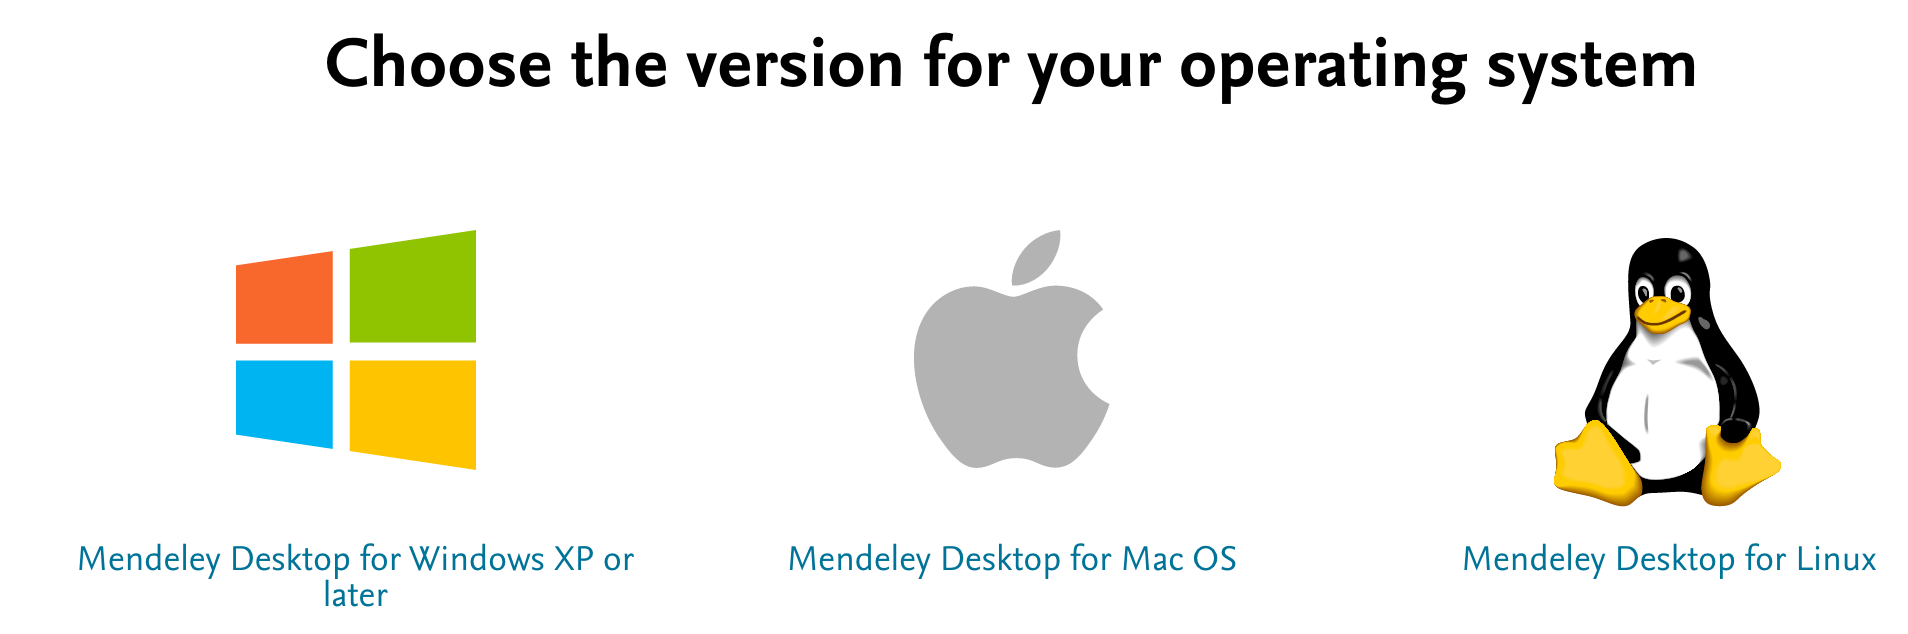
\includegraphics[width=12cm]{./image/desktop7.png}
\end{center}
앞 절에서 이야기한 웹에서 논문을 관리할 수 있는 것도 장점이지만 편하게 사용하고 싶다면, Desktop 프로그램이나 스마트폰용 APP을 활용할 수 있다. 인터넷이 연결된 환경에서 동기화만 시켜놓으면 인터넷 연결이 끊겨도 자유롭게 사용할 수 있다. 맨들리의 경우 windows와 Mac 모두 Desktop 프로그램을 무료로 제공하고 있는 점이 강점이다. 뒤에서 이야기할 친구들이나 선생님과 논문을 공유하는 경우 Mac을 사용하는 친구와 windows를 사용하는 친구 사이에서도 자유롭게 공유할 수 있다. 심지어 리눅스도 지원한다. \\
그럼 Desktop 프로그램을 다운로드하고 설치해보자.\\
\begin{tabular}{ m{11cm} m{50mm} }
	\hline
		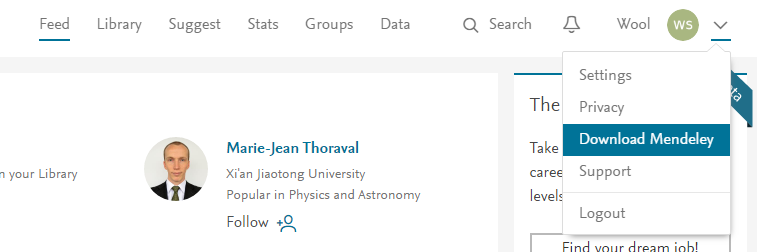
\includegraphics[width=10cm]{./image/desktop1.png}
	 & 맨들리 홈페이지에 접속한 다음 로그인 후, \textbf{Download Mendeley}를 클릭  \\
	\hline
	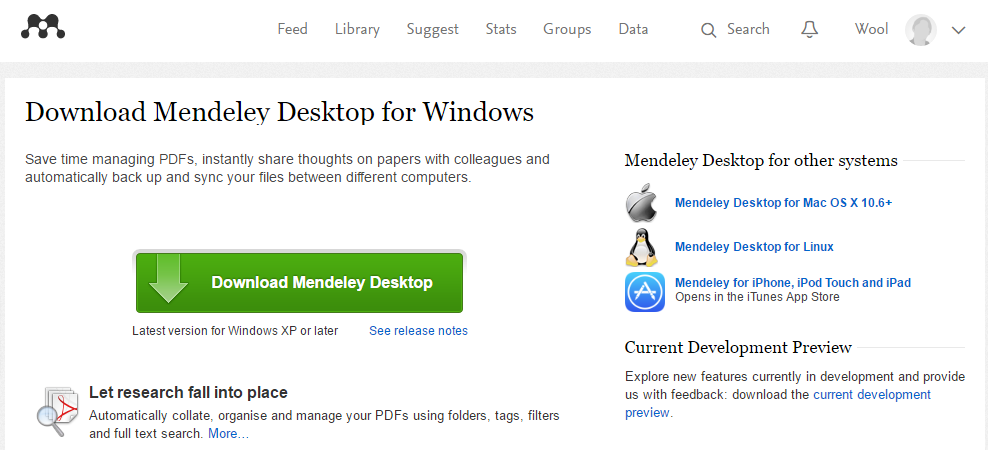
\includegraphics[width=10cm]{./image/desktop2.png} & 기본적으로 컴퓨터의 OS를 인식해서 OS별 설치파일을 다운로드할 수 있게 되어 있음. \textbf{Download Mendeley Desktop}을 클릭 \\
	\hline
	\centering
	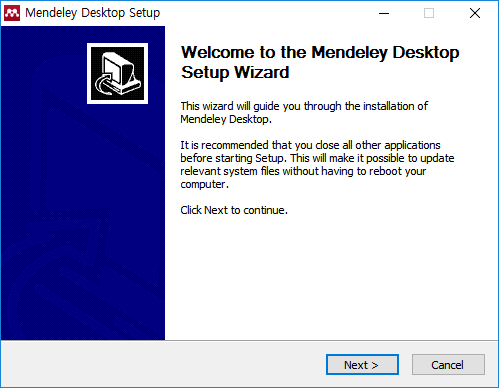
\includegraphics[width=7cm]{./image/desktop3.png} & 다운로드가 끝나면 설치파일을 실행해서 \textbf{Next}를 계속 클릭\footnote{광고나 다른 애드온 프로그램 없음} \\
\end{tabular} \\

\begin{tabular}{ m{11cm} m{50mm} }
	\hline
	\centering
	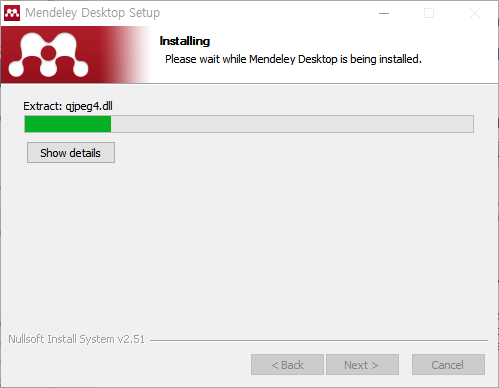
\includegraphics[width=7cm]{./image/desktop4.png} & 설치가 진행됨\\
	\hline
	\centering
	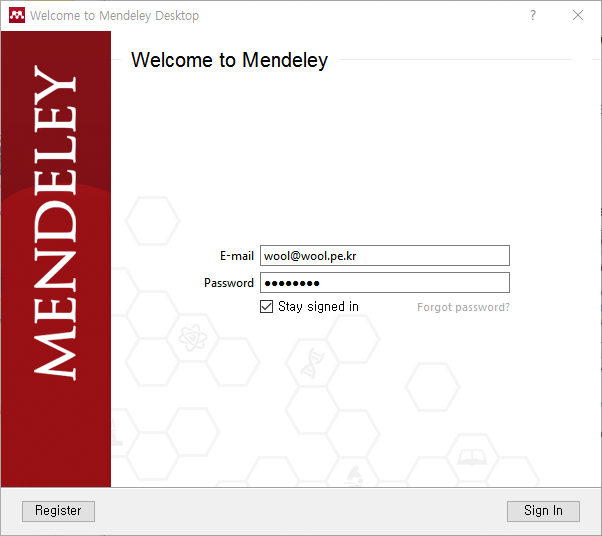
\includegraphics[width=7cm]{./image/desktop5.png} & 설치가 끝나면 로그인을 위해 계정 정보를 입력\\
	\hline
	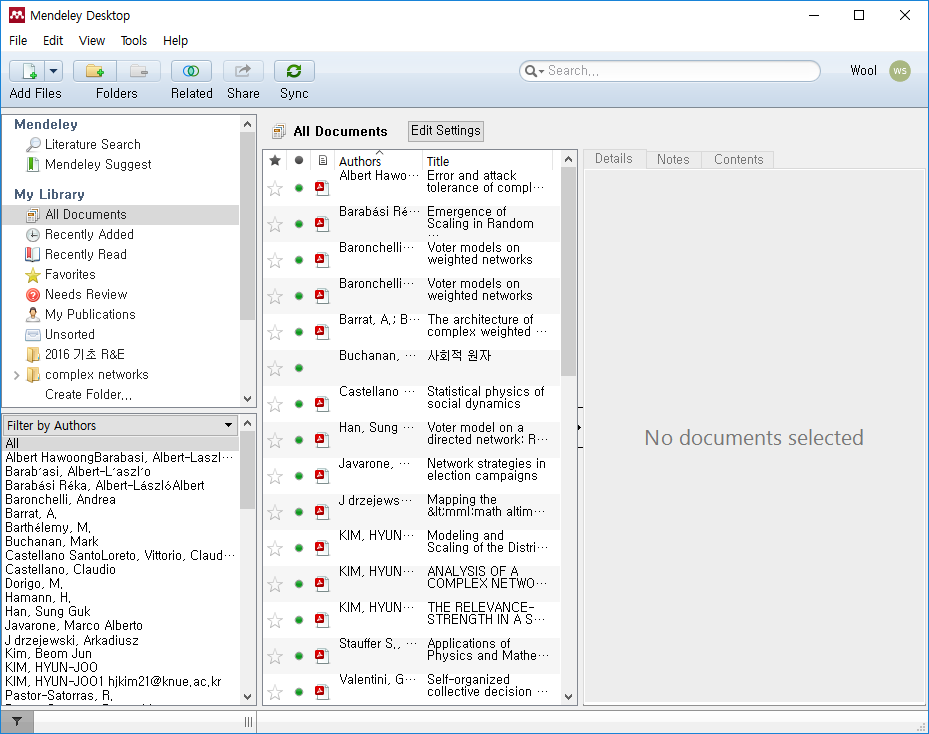
\includegraphics[width=10cm]{./image/desktop6.png} & Desktop이나 프로그램에서 \textbf{Mendeley}를 찾아서 실행\\
\end{tabular} \\
Desktop 프로그램 설치가 끝났다. 이제부터는 자유롭게 사용하면 되겠다.

\begin{center}
	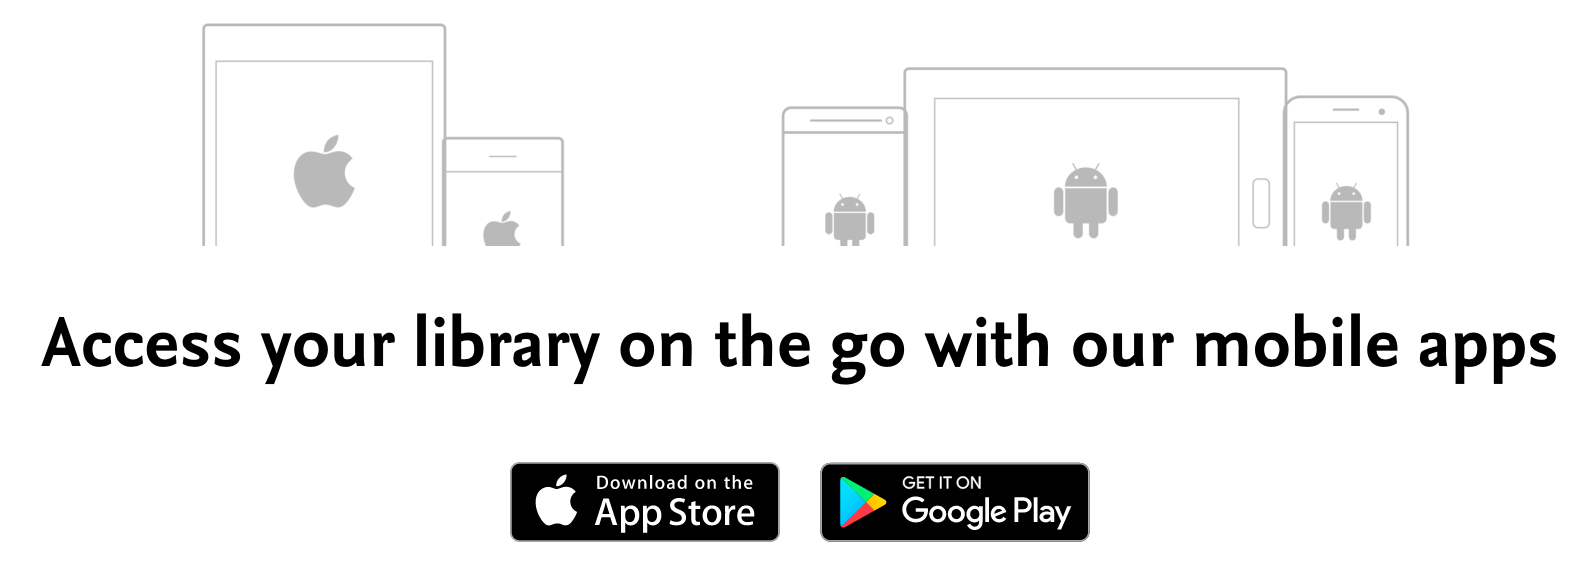
\includegraphics[width=12cm]{./image/desktop8.png}
\end{center}
스마트폰 OS도 iOS와 안드로이드를 모두 지원한다. 앱스토어나 구글플레이에서 \textrm{Mendeley} 검색한 후에 설치하고, 로그인하면 간편히 사용할 수 있다. 논문 원문을 첨부해뒀으면 싱크를 시키고 난 다음부터는 인터넷에 연결이 되지 않아도 확인할 수 있고, 간단히 형광펜으로 표시하는 정도의 Viewer를 제공한다.

\subsection{논문 추가하기}
학생들의 원활한 연구활동을 위해 학술데이터베이스를 많이 사용한다. RISS나 KISS도 있지만 학교에서는 DBpia(\textit{www.dbpia.co.kr})를 구독해 학교에서 자유롭게 사용할 수 있다.\footnote{교내에서는 별도의 인증없이 접속할 수 있으며, 구독이 끝나면 유료로 사용해야 한다.} DBpia에서 논문을 검색한 다음에 서지정보를 맨들리에 추가하는 방법은 다음과 같다. \\
\begin{tabular}{ m{11cm} m{50mm} }
	\hline
	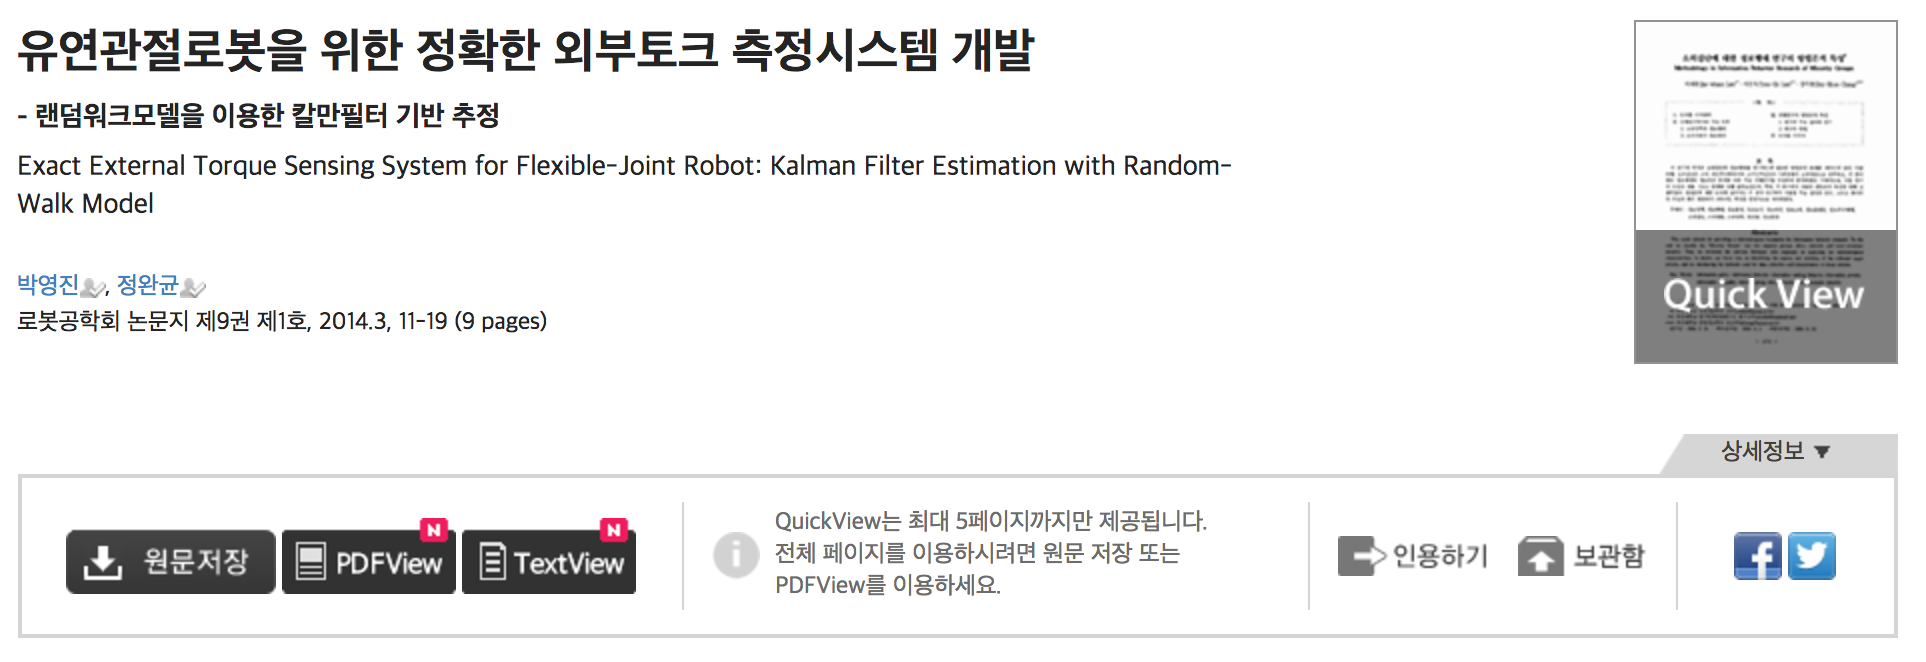
\includegraphics[width=10cm]{./image/ris_import1.png} & 논문을 검색 한 다음에 \textrm{인용하기}를 클릭\\
	\hline
	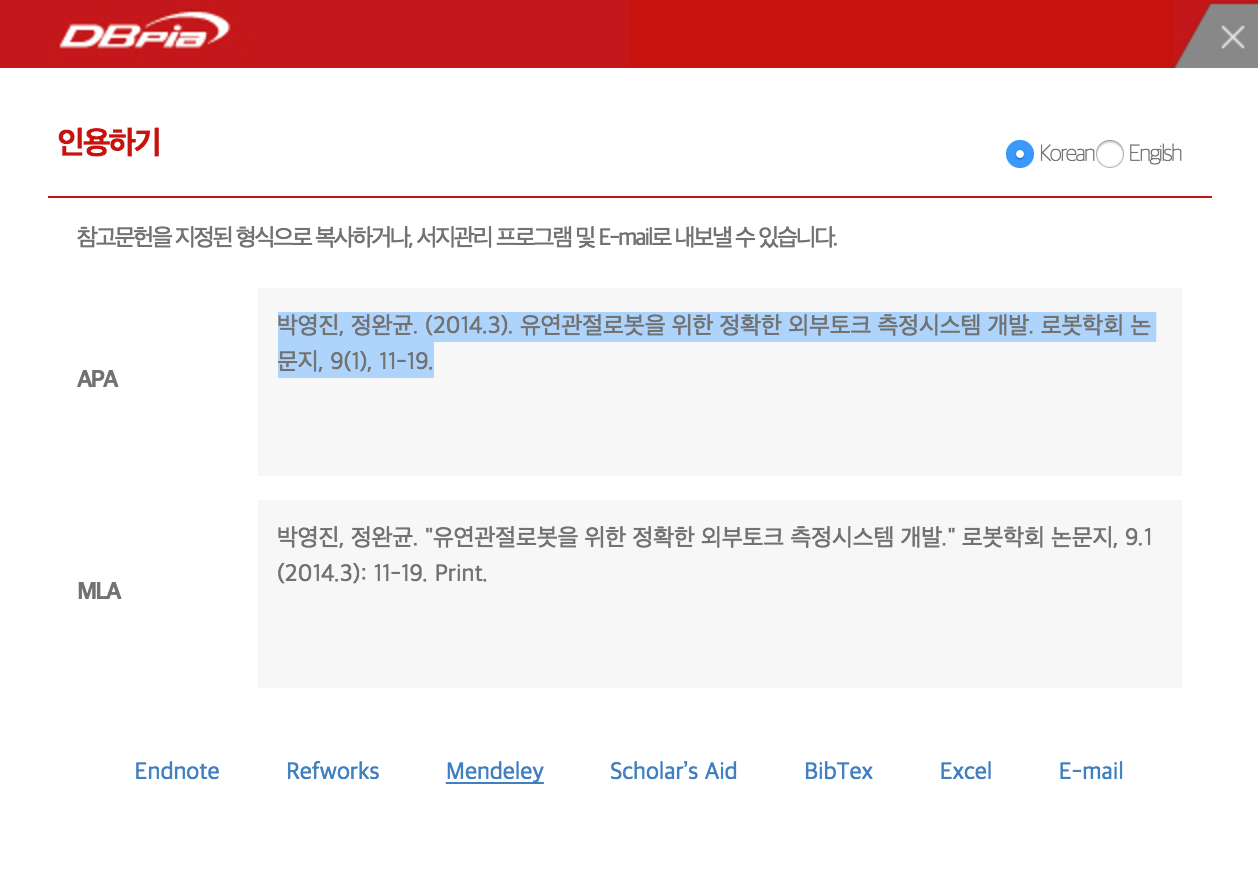
\includegraphics[width=10cm]{./image/ris_import3.png} & 아래에 보이는 서지관리 프로그램 중에서 \textrm{Mendeley}를 클릭\\

	
\end{tabular}

\begin{tabular}{ m{11cm} m{50mm} }
	\hline
	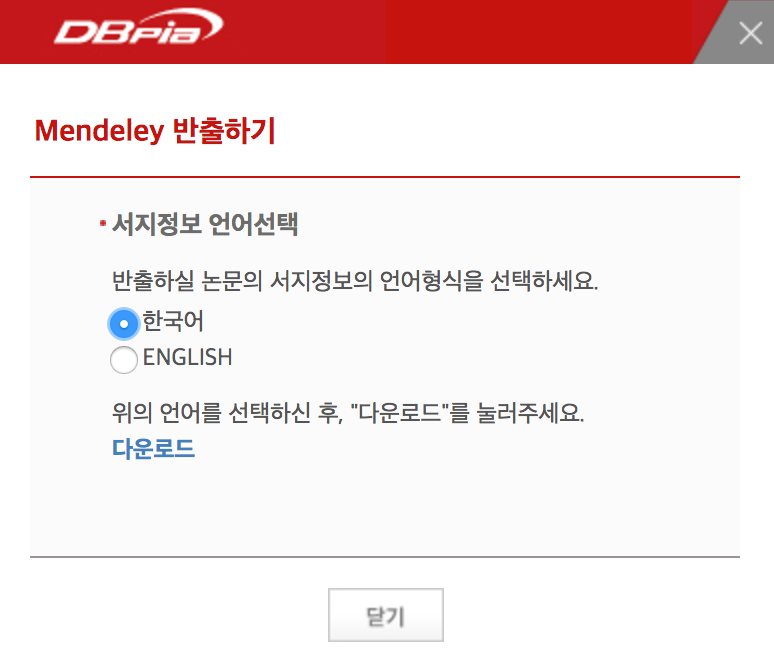
\includegraphics[width=7cm]{./image/ris_import4.png} & \textrm{다운로드}를 클릭해 \textit{*.ris} 파일이 저장\\
	\hline
	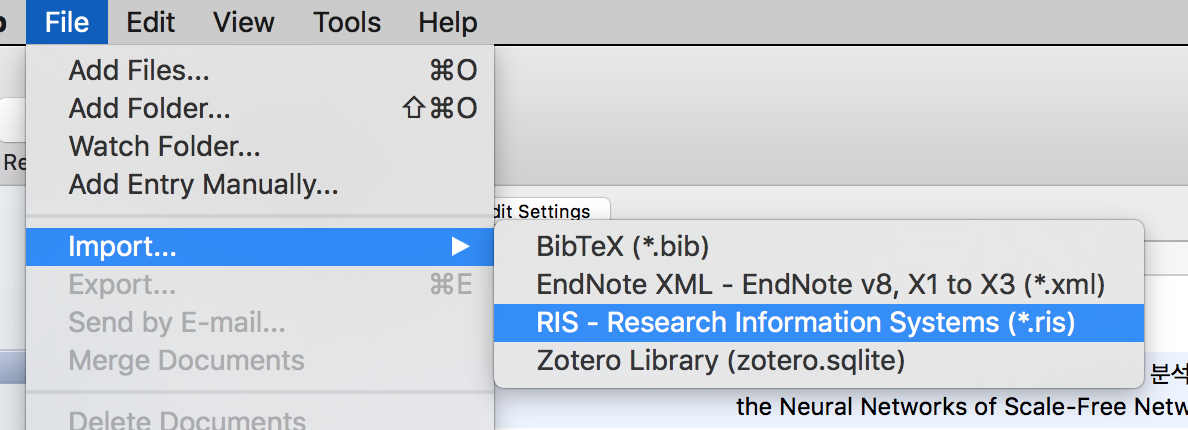
\includegraphics[width=10cm]{./image/ris_import5.png} & 맨들리를 실행한 뒤,  \textrm{File-Import-RIS}를 클릭해 앞에서 저장하 \textit{ris}파일을 불러옴 \\
	\hline
	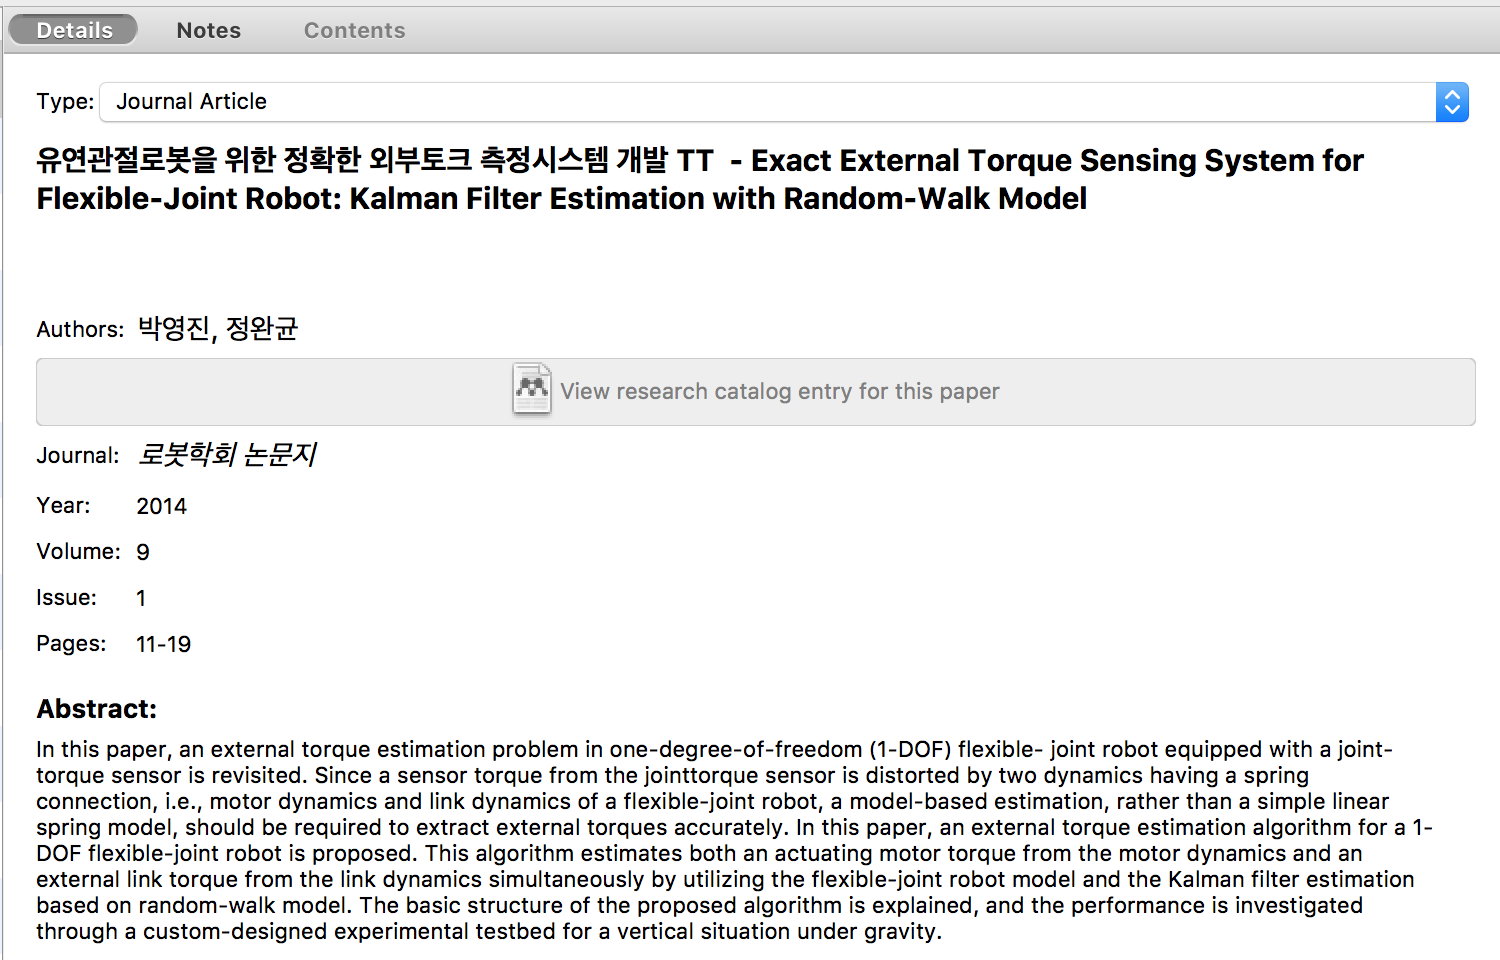
\includegraphics[width=10cm]{./image/ris_import7.png} & 맨들리에서 해당 논문을 선택하면 자세한 정보를 확인할 수 있음 \\
	\hline
	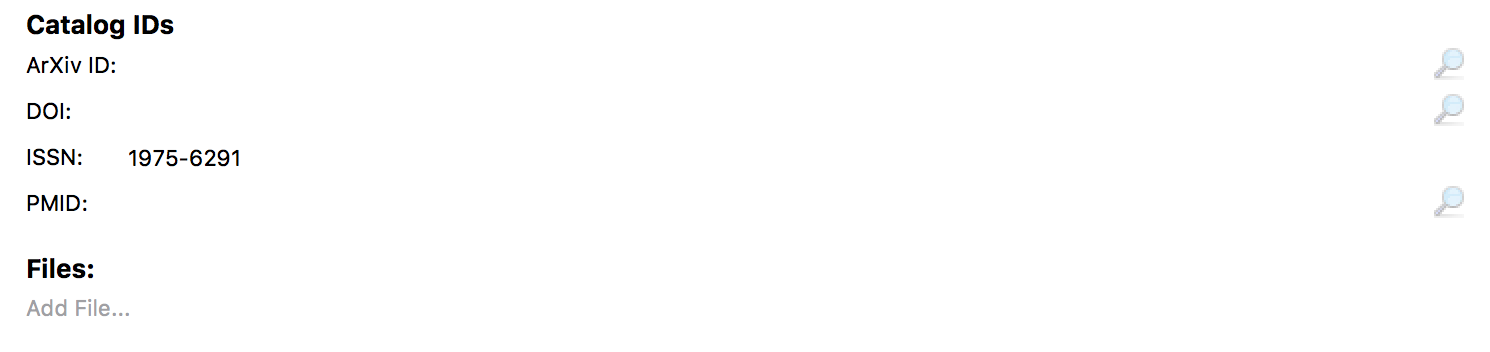
\includegraphics[width=10cm]{./image/ris_import8.png} & 추가로 논문 원문 PDF를 다운로드 했으면 아래에 보이는 \textrm{Add file}을 클릭해서 PDF를 추가\\
\end{tabular}

\newpage
\subsection{친구나 선생님과 목록 공유하기}
대부분의 연구활동은 모두 함께 진행된다. 맨들리는 손쉽게 문헌 목록들과 원문을 공유할 수 있도록 맨들리는 Group 기능을 제공한다. 간단히 Group을 만들고 친구나 선생님을 초대하면  된다.\\

\begin{tabular}{ m{11cm} m{50mm} }
	\hline
	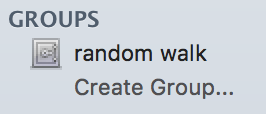
\includegraphics[width=5cm]{./image/group5.png} & 맨들리 Desktop에서 \textrm{Create Group}로 그룹을 만듦\\
	\hline
	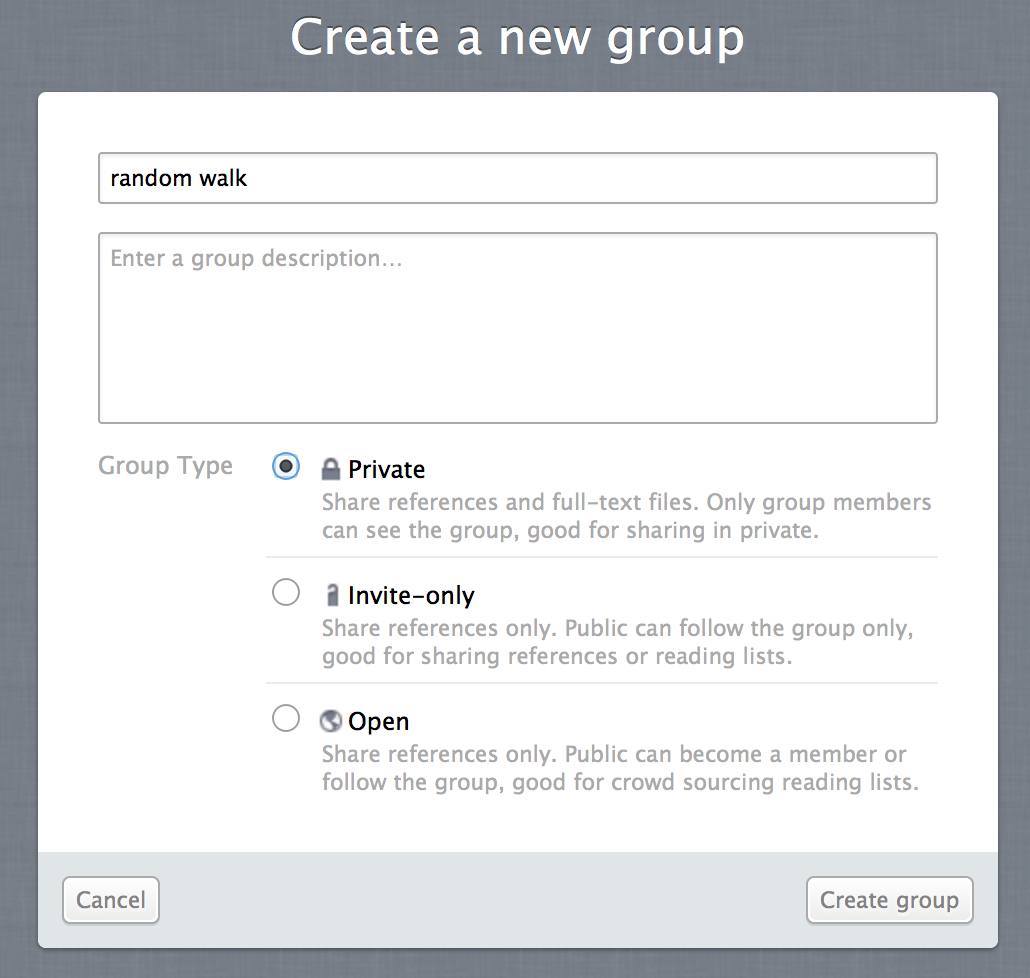
\includegraphics[width=8cm]{./image/group2.png} & \textrm{Create a new group}에서 그룹 이름을 입력하고, Type을 \textit{Private}으로 해야 멤버들과 모든 파일들을 함께 공유할 수 있음\\
	\hline
	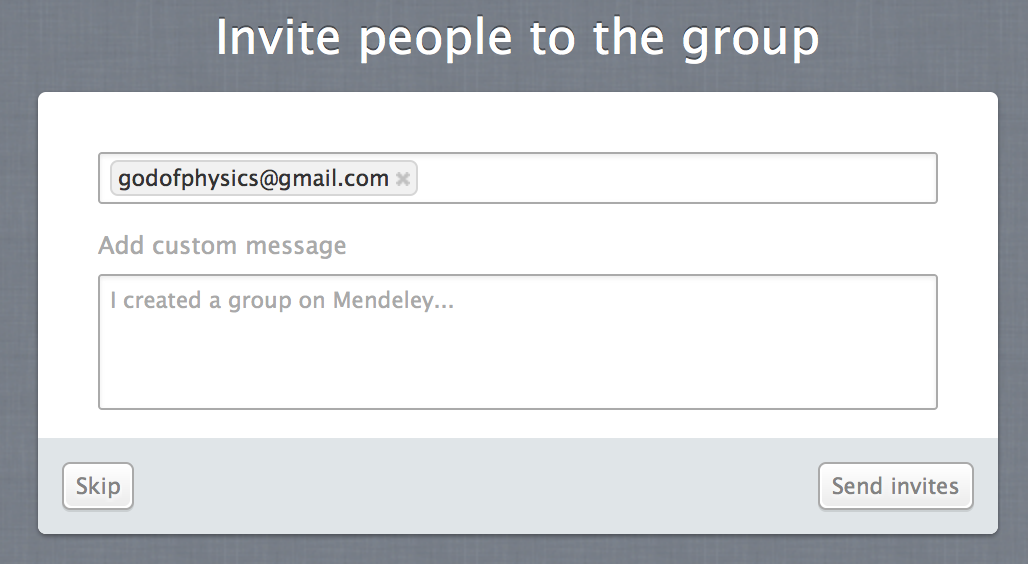
\includegraphics[width=8cm]{./image/group3.png} & 초대할 계정을 입력하고 초대\\
	\hline
	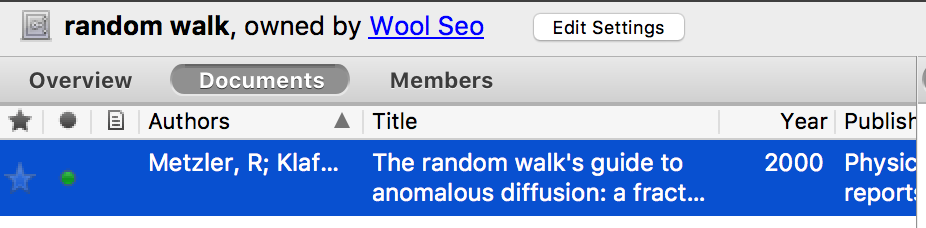
\includegraphics[width=8cm]{./image/group4.png} & 파일을 추가하고 활용\\
\end{tabular}

\newpage
\subsection{\LaTeX 연동해 Reference 만들기}
\LaTeX 을 사용하면 논문의 레퍼런스를 관리하기가 무척 쉽다. 특히 맨들리로 Bilbiography파일을 만든 다음에 \LaTeX 에서 필요한 곳에서 \textit{cite} 명령을 이용하면 쉽게 논문을 인용 표시할 수 있다. 무엇보다 가장 큰 장점은 순서에 맞춰 Reference를 자동으로 만들어 주는 것이다. 참고문헌이 10개가 넘는 글 중간에 새로운 참고문헌을 집어 넣어야 한다면 한글이나 워드는 하나하나 모두 찾아 수정해야 하지만, \LaTeX은 알아서 삽입해준다. \LaTeX이 궁금하다면 \textit{경기과학고 TEX 사용자협회}를 찾아보면 된다.\footnote{\textit{http://latex.gs.hs.kr/}} \\
간단히 순서를 설명하면 Reference에서 사용할 논문들을 선택해서 Bilbiography파일을 만들고, \LaTeX 에서 인용만 하면 된다.\\

\begin{tabular}[h]{ m{11cm} m{50mm} }
	\hline
	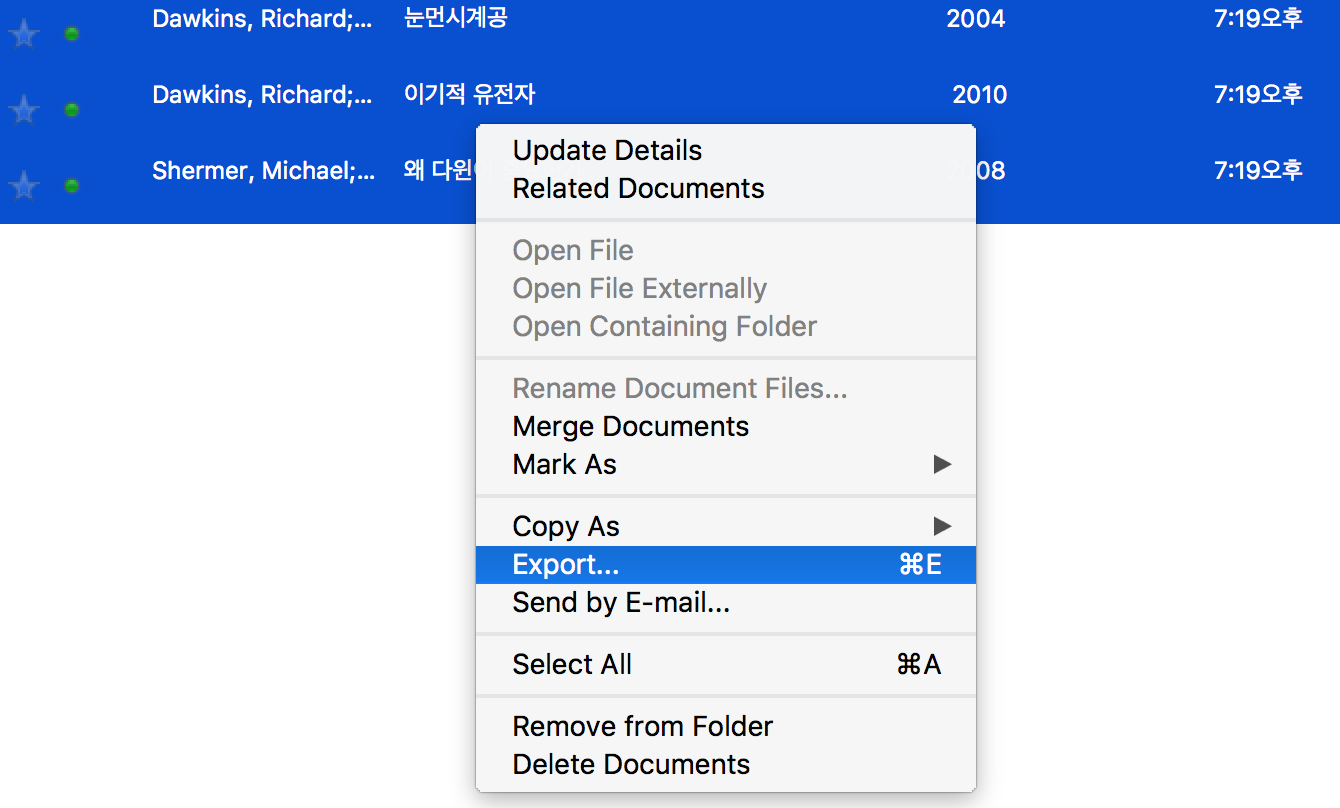
\includegraphics[width=10cm]{./image/latex_bibliography1.png} & 레퍼런스를 만들 논문들을 선택한 다음 \textit{Export}\\
	\hline
	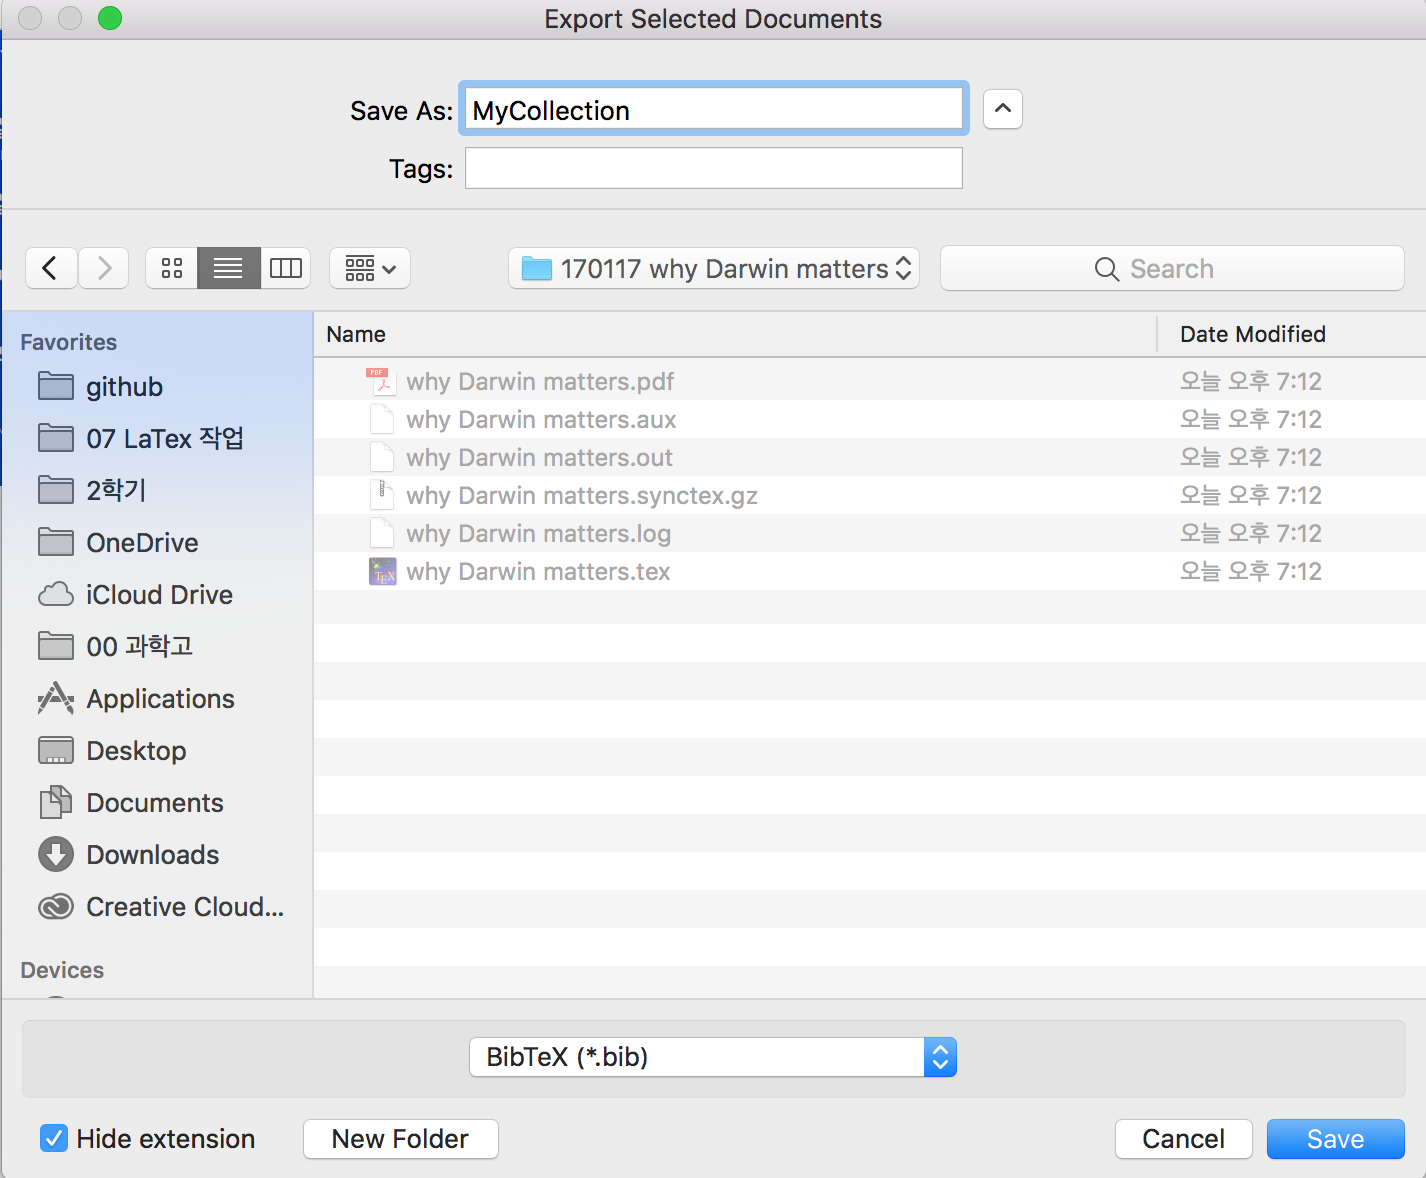
\includegraphics[width=10cm]{./image/latex_bibliography2.png} & 적당한 이름으로 저장\\
	\hline
	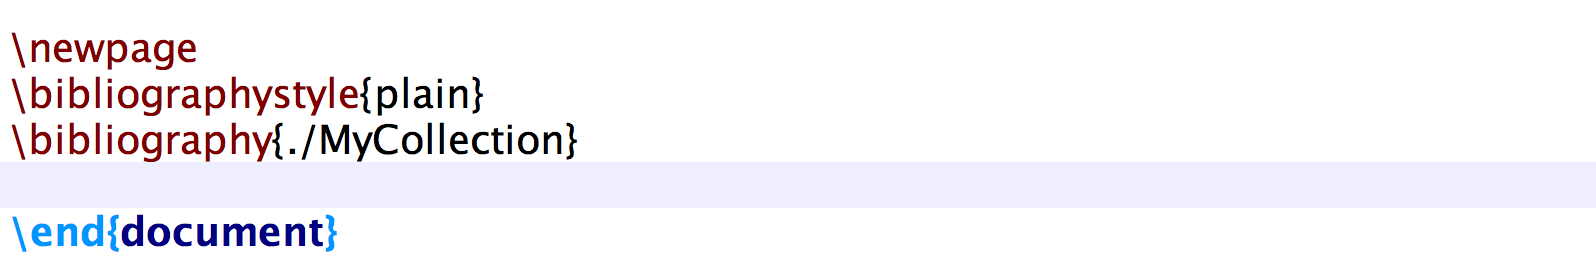
\includegraphics[width=10cm]{./image/latex_bibliography3.png} & \LaTeX에 다음 왼쪽의 코드를 레퍼런스가 들어갈 위치에 넣는다. \\
	\hline
	
\end{tabular}

\begin{tabular}{ m{11cm} m{50mm} }
	\hline
	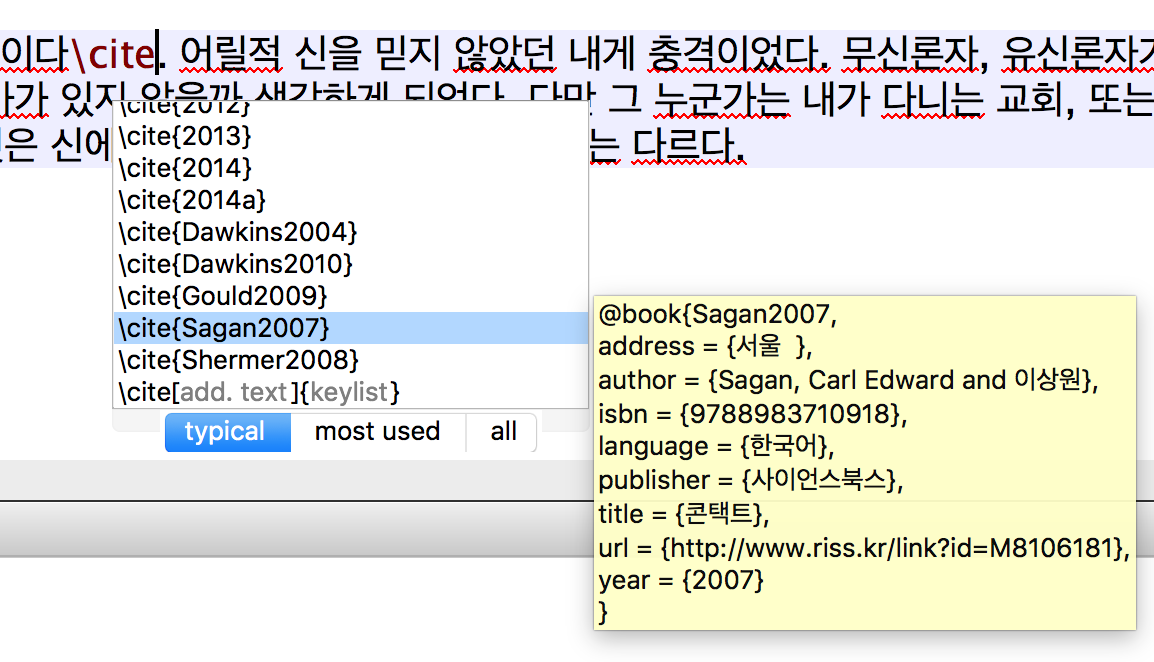
\includegraphics[width=10cm]{./image/latex_bibliography4.png} & 인용이 필요한 곳에서 \textit{cite}로 입력하면 인용 가능한 문헌 목록이 나타남 \\
	\hline
	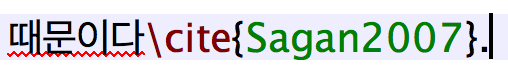
\includegraphics[width=10cm]{./image/latex_bibliography7.png} & 왼쪽과 같이 인용됨\\
	\hline
	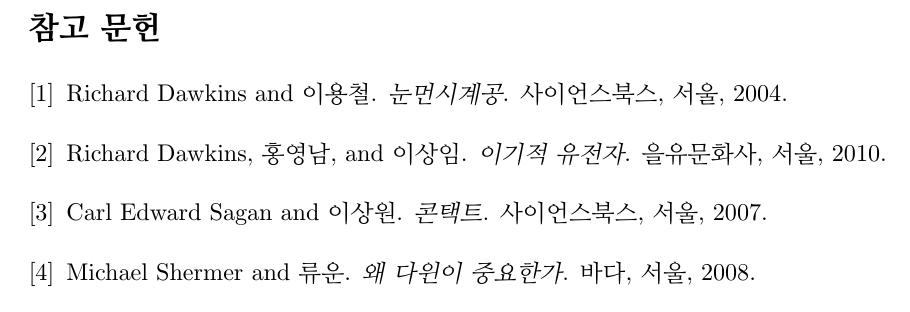
\includegraphics[width=10cm]{./image/latex_bibliography8.png} & 레퍼런스가 자동으로 나타남\\
\end{tabular}






\end{document}
